\documentclass[12pt]{article}
\usepackage[utf8]{inputenc}
\usepackage[T1]{fontenc}
\usepackage{amsmath}
\usepackage{amsfonts}
\usepackage{amssymb}
\usepackage[version=4]{mhchem}
\usepackage{stmaryrd}
\usepackage{graphicx}
\usepackage{chemformula}
\graphicspath{ {./images/} }

\usepackage{listings} % Required for insertion of code
\usepackage{xcolor} % Required for custom colors

% Define custom colors
\definecolor{codegreen}{rgb}{0,0.6,0}
\definecolor{codegray}{rgb}{0.5,0.5,0.5}
\definecolor{codepurple}{rgb}{0.58,0,0.82}
\definecolor{backcolour}{rgb}{0.95,0.95,0.92}

% Setup the style for code listings
\lstdefinestyle{mystyle}{
    backgroundcolor=\color{backcolour},   
    commentstyle=\color{codegreen},
    keywordstyle=\color{magenta},
    numberstyle=\tiny\color{codegray},
    stringstyle=\color{codepurple},
    basicstyle=\ttfamily\footnotesize,
    breakatwhitespace=false,         
    breaklines=true,                 
    captionpos=b,                    
    keepspaces=true,                 
    numbers=left,                    
    numbersep=5pt,                  
    showspaces=false,                
    showstringspaces=false,
    showtabs=false,                  
    tabsize=2
}

% Activate the style
\lstset{style=mystyle}


\title{Chemistry 14 (Spring term 2024) \\
 Midterm Examination }


\author{Distributed Thursday, May 2, 2024\\
Due $\quad$ Thursday, May 9, 2024 by 11:59 pm uploaded through Canvas}
\date{}


\begin{document}
\maketitle


\section*{Conditions}
\begin{itemize}
  \item Open the midterm examination pdf when you are ready to take it.

  \item You have 4 hours to complete this examination (excluding a short break).

  \item You may use the Ch14 online lecture notes, problem sets and solutions, the course web site and a calculator. You may also use the Harris \& Lucy text (or earlier editions). You may also use handwritten notes you have made from other books. You may not discuss the exam with others, use any other books (including those on Reserve), or other web sites.

  \item You may use Mathematica $®$, Matlab®, Excel® or equivalent program to get numerical solutions, including solving polynomial equations. Please note, though, that the problems can be worked with a quadratic equation as the most complex equation that needs to be solved.

  \item Write your answers in the same sequential order as in the exam.

  \item After you have finished the exam, upload your answers through Canvas, just as you do for the problem sets.

  \item Show your work! Getting the right answer is not enough - the intermediate steps are needed for credit. If you use Mathematica $\circledR$ or related program to get numerical solutions, be sure to clearly write out in the exam the specific equation being solved. Note: you do not need to derive equations that were derived in class.

  \item Unless otherwise instructed, you should report answers to 3 significant figures and assume that activities can be approximated by concentrations. You may use approximate formulas as long as you justify the particular approximation (ie in a sufficiently acidic solution, $\left(\mathrm{OH}^{-}\right)$may be neglected relative to $\left(\mathrm{H}^{+}\right)$, etc).

\end{itemize}

\section*{unless otherwise stated, you may assume:}
aqueous solutions

$\mathrm{T}=298.15 \mathrm{~K}=25^{\circ} \mathrm{C}$

$P=1$ atm

$R=8.3144 \mathrm{~J} \mathrm{~mol}^{-1} \mathrm{~K}^{-1}=0.08206$ liter atm $\mathrm{mol}^{-1} \mathrm{~K}^{-1}$

$\mathrm{K}_{w}=10^{-14}$

Debye-Huckel limiting expression, water, $25^{\circ} \mathrm{C}$

individual ionic activity coefficient $\log \gamma_{i}=-0.509 z_{i}^{2} \sqrt{I}$

mean ionic activity coefficient $\quad \log \gamma_{ \pm}=-0.509\left|z_{+} z_{-}\right| \sqrt{I}$

\section*{Chemistry 14 (Spring term 2024)}
Midterm Examination

\begin{center}
\begin{tabular}{lrl}
problem & points &  \\
1a & 5 &  \\
1b & 5 & $\square$ \\
2a & 10 &  \\
$2 b$ & 10 & $\square$ \\
3a & 5 &  \\
3b & 10 & $\square$ \\
3c & 10 & $\square$ \\
3d & 10 & $\square$ \\
3e & 10 & $\square$ \\
4a & 10 &  \\
4b & 10 & $\square$ \\
5 & 5 &  \\
 &  &  \\
total & 100 &  \\
\end{tabular}
\end{center}

\section{Strong acids and strong bases}
Nitric acid is a strong acid and barium hydroxide is a strong base. Assume activities equal concentrations in this problem.

\subsection{}
Calculate the $\mathrm{pH}$ of solution containing $0.001 \mathrm{M}$ barium hydroxide $\left(\mathrm{Ba}(\mathrm{OH})_{2}\right)$.
\subsubsection{Answer}
\begin{align*}
  \ce{Ba(OH)2 &-> Ba^2+ + 2OH-} \\
  \ce{[Ba(OH)2] & = 0.001 M} -> \ce [OH-] = 0.002 M \\
  \ce{Kw & = [H+][OH-]} = 10^{-14} \\
  \ce{[H+] & = \frac{10^{-14}}{0.002}} = 5 \times 10^{-12} \\
  \ce{pH & = -\log[H+]} = 11.3
\end{align*}

\subsection{}

Calculate the $\mathrm{pH}$ of a solution containing $0.1 \mathrm{M}$ barium nitrate $\left(\mathrm{Ba}\left(\mathrm{NO}_{3}\right)_{2}\right)$.
\subsubsection{Answer}
$\left(\mathrm{Ba}\left(\mathrm{NO}_{3}\right)_{2}\right)$ is a salt of a strong acid and a strong base, so it will not affect the $\mathrm{pH}$ of the solution. The $\mathrm{pH}$ of the solution will be the same as the $\mathrm{pH}$ of the water, which is 7.

\section{Weak acids and weak bases}
\subsection{}
Sulfuric acid completely dissociates to $\mathrm{H}^{+}$and $\mathrm{HSO}_{4}^{-}$in solutions more dilute than $0.1 \mathrm{M} . \mathrm{HSO}_{4}$ - further dissociates to $\mathrm{H}^{+}$and $\mathrm{SO}_{4}{ }^{2-}$ with $\mathrm{K}_{\mathrm{a}}=1.02 \times 10^{-2}$. Calculate the $\mathrm{pH}$ of a $0.05 \mathrm{M}$ solution of sulfuric acid. Since sulfuric acid is both a strong acid and a weak acid, start with the charge balance equation for this system. Assume activities equal concentrations.
\subsubsection{Answer}
We are interested in the two dissociation expressions for sulfuric acid:
\begin{align*}
  \ce{H2SO4 &-> H+ + HSO4-} with Ka = \infty \\
  \ce{HSO4- &-> H+ + SO4^2-} with Ka = 1.02 \times 10^{-2}
\end{align*}
We initially know that the concentration of protons is equal to the concentration of sulfuric acid, so $[H+] = 0.05 M$ and $[HSO4-] = 0.05 M$. We can then use the second dissociation to find the concentration of $[SO4^2-]$:
\begin{align*}
  \ce{HSO4- &-> H+ + SO4^2-} \\
  \ce{Ka & = \frac{[H+][SO4^2-]}{[HSO4-]}} \\
\end{align*}
Let us set the parameter $x$ to be the concentration of $[SO4^2-]$. Than the final concentration of $[HSO4-]$ will be $0.05 - x$ and the final concentration of $[H+]$ will be $0.05 + x$. We can then solve for $x$. This suggests the expression:
\begin{align*}
  1.02 \times 10^{-2} & = \frac{(0.05 + x)x}{0.05 - x} \\
\end{align*}
Solving gives a solution for $x$ as 0.00753 M. This means that the concentration of $[H+]$ is $0.05 + 0.00753 = 0.05753 M$. The $\mathrm{pH}$ is then $-\log(0.05753) = 1.24$.
% Inline Python code in the document
\begin{lstlisting}[language=Python]
from sympy import symbols, Eq, solve

# Define the variable
x = symbols('x', real=True, positive=True)

# Given constants
Ka2 = 1.02e-2
initial_H2SO4 = 0.05  # Initial concentration of H2SO4 and hence HSO4-

# Ka expression for the second dissociation of HSO4-
equation_Ka = Eq((initial_H2SO4 + x) * x / (initial_H2SO4 - x), Ka2)

# Solve the equation
x_value = solve(equation_Ka, x)
x_value
\end{lstlisting}
\subsection{}
Calculate the $\mathrm{pH}$ and the equilibrium concentrations of $\left(\mathrm{NH}_{3}\right)$ and $\left(\mathrm{NH}_{4}{ }^{+}\right)$ present in a solution of $\mathrm{NH}_{3}$ made to a total concentration of $1.0 \times 10^{-6} \mathrm{M}\left(=\left(\mathrm{NH}_{3}\right)+\right.$ $\left(\mathrm{NH}_{4}+\right.$ )). The $\mathrm{pK}_{b}$ of $\mathrm{NH}_{3}=4.75$. Assume activities equal concentrations. Although this is a dilute $\mathrm{NH}_{3}$ solution, you can reasonably neglect $\left(\mathrm{H}^{+}\right)$in the charge balance equation.
\subsubsection{Answer}
We are interested in the expression for the equilibrium of $\ce{NH3}$ in water:
\begin{align*}
  \ce{NH3 &-> NH4+ + OH-} \\
  \ce{Kb & = \frac{[NH4+][OH-]}{[NH3]}} \\
\end{align*}
We know the pKb of $\ce{NH3}$ is 4.75, so the Kb is $10^{-4.75}$. The fervent verbose that we want to set up is the parameter $x$ to be the concentration of $[OH-]$ and $[NH4+]$ which will be present in equal amounts. If we were to set up a charge balance equation for this process, it would reflect this tract. The final concentration of $[NH3]$ will be $1.0 \times 10^{-6} - x$. This suggests the expression:
\begin{align*}
  10^{-4.75} & = \frac{x^2}{1.0 \times 10^{-6} - x} \\
\end{align*}
Solving for $x$ gives a value of 9.49 $\times 10^{-7} M$.
% Inline Python code in the document
\begin{lstlisting}[language=Python]
from sympy import symbols, Eq, solve, log

# Define the variable
x = symbols('x', real=True, positive=True)

# Given constants
Kb = 10**(-4.75)
initial_NH3 = 1.0e-6  # Total initial concentration of NH3

# Kb expression for the reaction
equation_Kb = Eq(x**2 / (initial_NH3 - x), Kb)

# Solve the equation for x
x_value = solve(equation_Kb, x)
x_value
\end{lstlisting}
So the equilibrium concentrations of $\left(\mathrm{NH}_{4}{ }^{+}\right)$ is $9.49 \times 10^{-7} M$. And that of $\left(\mathrm{NH}_{3}\right)$ is $1.0 \times 10^{-6} - 9.49 \times 10^{-7} = 0.51 \times 10^{-7} M$. The $\mathrm{pOH}$ is $-\log(9.49 \times 10^{-7}) = 6.02$ and the $\mathrm{pH}$ is $14 - 6.02 = 7.98$.






\section{Maintaining a buffer}
\subsection{}
The titration curve of glycine was discussed in lecture 8. The pKa's of glycine are $\mathrm{pK}_{1}=2.35$ and $\mathrm{pK}_{2}=9.78$, respectively. Is glycine a better buffer when $\mathrm{pH}=$ $\mathrm{pK}_{1}$ or when the $\mathrm{pH}$ equals the isoelectric point ( $\mathrm{pl}$ ) of glycine? Explain briefly.
\subsubsection{Answer}
We are given in the lecture that at the isoelectric point, the $[H^+] = \sqrt{K_1K_2}$. This translates to an averaged out pH of 6.07, and is the point where it is in the zwitterionic form. The lecture notes also give that the better buffer exist when the pH is closer to the pKa values. When this is the case, the glycine has a better chance to both accept and donate protons, and hence act as a better buffer. This means that glycine is a better buffer when the pH equals the pKa values of glycine, in this case, when the pH equals $\mathrm{pK}_{1}$.

\subsection{}


What are the fractions of glycine with 0, 1, and 2 protons bound in a solution of glycine when $\mathrm{pH}=\mathrm{pK}_{2}$? Assume activities equal concentrations.
\subsubsection{Answer}
We are interested in the quantity:
\begin{equation}
  \bar{h} = \frac{K_1 [H^+] + 2K_1K_2}{[H^+]^2 + K_1[H^+] + K_1K_2}
\end{equation}
We know that the pH is equal to the pK2, so the concentration of protons is equal to $10^{-9.78}$. We can then substitute this value into the equation.

As given in the lecture, the fractions of each form of glycine are given by:
\begin{align*}
  f_{\ch{H2A+}} &= \frac{[H^+]^2}{[H^+]^2 + K_1 [H^+] + K_1 K_2}, \\
  f_{\ch{HA}} &= \frac{K_1 [H^+]}{[H^+]^2 + K_1 [H^+] + K_1 K_2}, \\
  f_{\ch{A-}} &= \frac{K_1 K_2}{[H^+]^2 + K_1 [H^+] + K_1 K_2}.
\end{align*}

Because the last two fractions are the same, they give values of 0.5 and then because the K2 = $[H^+]$ is much smaller than the K1, the fraction of glycine with 0 protons is much smaller so we can approximate it as 0. The fractions of glycine with 0, 1, and 2 protons bound are 0, 0.5, and 0.5, respectively.
% Inline Python code in the document
\begin{lstlisting}[language=Python]
import math

# Constants
pK1 = 2.35
pK2 = 9.78

# Equilibrium constants
K1 = 10**(-pK1)
K2 = 10**(-pK2)

# Proton concentration at pH = pK2
H_plus = 10**(-pK2)

# Fractions of each form of glycine
f_H2A_plus = H_plus**2 / (H_plus**2 + K1 * H_plus + K1 * K2)
f_HA = K1 * H_plus / (H_plus**2 + K1 * H_plus + K1 * K2)
f_A_minus = K1 * K2 / (H_plus**2 + K1 * H_plus + K1 * K2)

print(f"Fraction of H2A+ (glycine with 2 protons): {f_H2A_plus:.4f}")
print(f"Fraction of HA (glycine with 1 proton): {f_HA:.4f}")
print(f"Fraction of A- (glycine with 0 protons): {f_A_minus:.4f}")
\end{lstlisting}


3c. (10 pts) What are the concentrations of $\mathrm{HAc}$ and $\mathrm{Ac}^{-}$in a $0.1 \mathrm{M}$ acetate buffer (ie, $\left.(\mathrm{HAc})+\left(\mathrm{Ac}^{-}\right)=0.1 \mathrm{M}\right)$ at $\mathrm{pH} 4.76$ ? The pKa of HAc is 4.76 . Assume activities equal concentrations.

3d. (10 pts) Calculate the volumes of glacial acetic acid (17.4 M) and $2.54 \mathrm{M} \mathrm{NaOH}$ needed to make 2 liters of $0.2 \mathrm{M}$ acetate buffer, pH 5.0 (ie, $\left.(H A c)+\left(A c^{-}\right)=0.2 M\right)$. Assume activities equal concentrations.\\
3e. (10 pts) A citrate buffer is made up of $0.01 \mathrm{M} \mathrm{Na}_{2} \mathrm{H}$ citrate and $0.01 \mathrm{M} \mathrm{Na}_{3}$ citrate, where the relevant $\mathrm{pK}_{3}=6.40$ for this reaction:

$$
\text { Hcitrate }^{2-} \stackrel{K_{3}}{\rightleftharpoons} \text { citrate }^{3-}+H^{+}
$$

Using the Debye-Huckel limiting law and the Henderson-Hasselbalch equation, estimate the actual $\mathrm{pH}$ of this buffer. You can neglect the contribution of $\mathrm{H}+$ and $\mathrm{OH}-$ to the ionic strength.

(citrate is a tricarboxylic acid with the following structure:

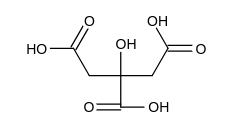
\includegraphics{smile-lvslvvf9smi5kvdw2w.png}


Hcitrate ${ }^{2-}$ and citrate ${ }^{3-}$ have 2 and 3 dissociated protons, respectively.)

\section*{Problem 4. Keep your equilibrium - it's a gas.}
The gases $\mathrm{N}_{2} \mathrm{O}_{4}$ and $\mathrm{NO}_{2}$ interconvert through the following equilibrium

$$
\mathrm{N}_{2} \mathrm{O}_{4} \stackrel{K_{p}}{\rightleftharpoons} 2 \mathrm{NO}_{2}
$$

4a. (10 pts) The free energies of formation at $298 \mathrm{~K}$ for $\mathrm{N}_{2} \mathrm{O}_{4}$ and $\mathrm{NO}_{2}$ are 99.8 and $51.3 \mathrm{~kJ} \mathrm{~mol}^{-1}$, respectively. Calculate the equilibrium constant $\mathrm{K}_{\mathrm{p}}$ for this reaction at 298

K.

4b. (10 pts) What are the partial pressures of $\mathrm{N}_{2} \mathrm{O}_{4}$ and $\mathrm{NO}_{2}$ (in atm) at equilibrium when the total pressure is $1 \mathrm{~atm}$ ? If you are unsure of your answer to $4 \mathrm{a}$, you may use Keq $=1$ (accurate to within a factor of 100 )

\section*{Problem 5. Getting blasted}
\begin{enumerate}
  \setcounter{enumi}{4}
  \item ( $5 \mathrm{pts}$ ) What is the role of the argon plasma in the inductively coupled plasma mass spectrometry (ICP-MS) instrument we discussed in the Water and Environment Laboratory tour?
\end{enumerate}

\end{document}